\chapter{Supply-Chain Risk Governance}
\section{Vendor Vulnerability Matrix}
Internal Make ownership eliminates commercial SaaS renewal escalation, while shifting security hardening and continuity risk onto the hosting organization. Auditing \textit{SyncFlow}'s codebase alongside vendor terms identified eleven concrete risks scored on a $5 \times 5$ \textbf{Likelihood ($P$) $\times$ Impact ($I$)} grid ($1 = \text{Low}$, $25 = \text{Critical}$).

\begin{figure}[H]
    \centering
    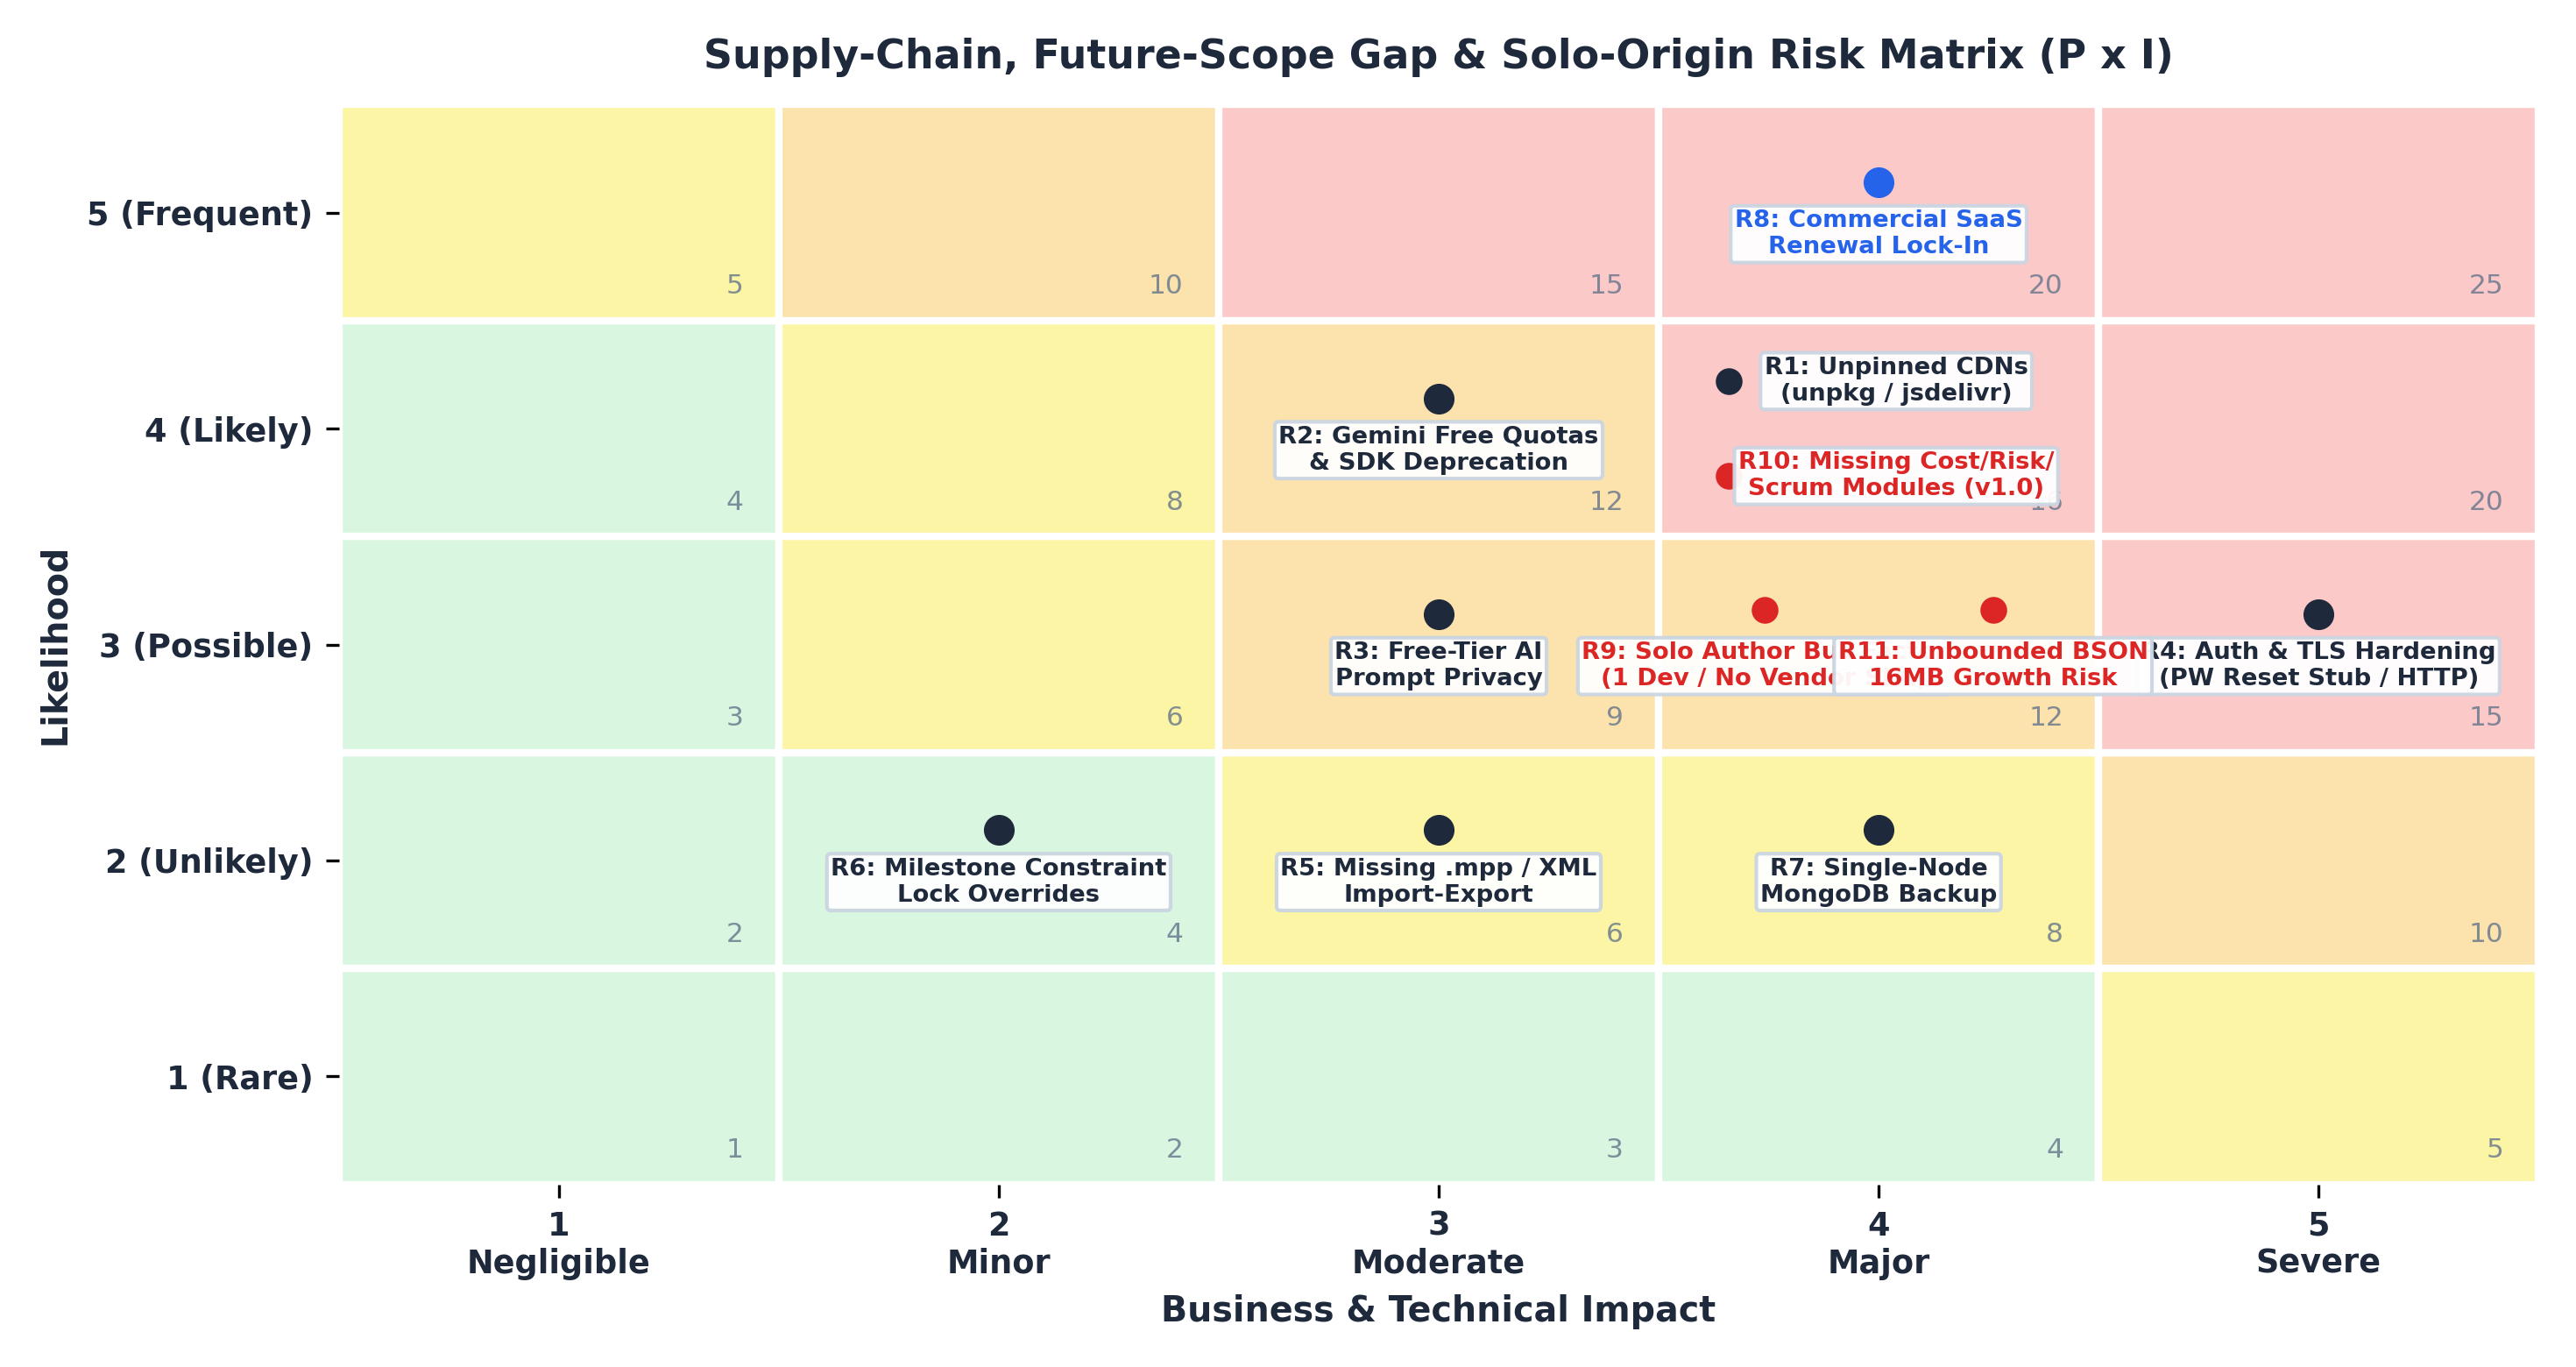
\includegraphics[width=0.95\textwidth]{images/va_risk_heatmap.png}
    \caption*{Five-by-five risk heatmap combining SyncFlow repository, Future-Development scope gaps, solo-author and data scaling risks ($R_1$--$R_7, R_9\text{--}R_{11}$) against commercial SaaS escalation ($R_8$).}
\end{figure}

\begin{table}[H]
\centering
\tiny
\renewcommand{\arraystretch}{1.18}
\caption*{Consolidated Risk Register Covering Supply-Chain, Future-Scope Gaps, Continuity, and Scalability.}
\begin{tabularx}{\textwidth}{l l c c c X}
\toprule
\textbf{ID} & \textbf{Risk Event} & \textbf{$P$} & \textbf{$I$} & \textbf{$P \times I$} & \textbf{Technical Root Cause / Concrete Mitigation Control} \\
\midrule
$R_8$ & Commercial SaaS Price Escalation & $5$ & $4$ & $20$ & Recurring renewal hikes across commercial SaaS and commercialized \textit{SyncFlow SaaS}. Avoided under internal Make hosting. \\
$R_1$ & Unpinned Frontend CDN Imports & $4$ & $4$ & $16$ & HTML fetches unpinned CDN script tags. An external outage breaks charts. Fix: vendor static assets locally. \\
$R_{10}$ & Missing Cost/Risk/Scrum Pillars & $4$ & $4$ & $16$ & \textit{SyncFlow v1.0} lacks monetary Cost, Risk + Monte Carlo, and Scrum sprints. Resolved across the planned \textit{v2.0} upgrades. \\
$R_4$ & Auth, TLS Hardening Gaps & $3$ & $5$ & $15$ & Missing SMTP password-reset delivery and plain HTTP container setup. Fix: 36h Caddy Server 2 TLS, JWT, and SMTP sprint. \\
$R_9$ & Solo-Author Bus Factor & $3$ & $4$ & $12$ & Single original maintainer with no external vendor SLA. Fix: modular docs, CI tests, and secondary maintainer onboarding. \\
$R_{11}$ & Unbounded BSON Growth (16\,MB Limit) & $3$ & $4$ & $12$ & Storing continuous timer logs and baselines inside a single project document risks reaching MongoDB's 16\,MB limit. Fix: extract into dedicated referenced collections in \textit{v2.0}. \\
$R_2$ & Gemini Free Quotas, SDK Shift & $4$ & $3$ & $12$ & Free AI Studio keys face \texttt{429} throttling and legacy SDK deprecation. Fix: migrate to \texttt{google-genai} SDK. \\
$R_3$ & Free-Tier AI Prompt Privacy & $3$ & $3$ & $9$ & Unpaid AI API tiers may log prompts under public terms. Fix: use paid Tier-1 billing (€120 budgeted) or run offline. \\
$R_7$ & Single-Node MongoDB Backup & $2$ & $4$ & $8$ & Single database volume creates recovery exposure. Fix: daily encrypted off-site \texttt{mongodump} backups (€6/mo budgeted). \\
$R_5$ & Missing MS Project XML Export & $2$ & $3$ & $6$ & Lack of \texttt{.mpp}/\texttt{.xml} and PDF audit exports hinders executive sharing. Addressed inside the planned \textit{v2.0} interoperability scope. \\
$R_6$ & Milestone Constraint Overrides & $2$ & $2$ & $4$ & The 14-point audit engine actively checks Metric~5 in \textit{v1.0}. Interactive UI date locks for individual milestone overrides expand in planned \textit{v2.0}. \\
\bottomrule
\end{tabularx}
\end{table}

\newpage

\section{Weight Sensitivity Validation}
Sensitivity testing confirms that \textit{SyncFlow v2.0 (Make)} leads three of four procurement scenarios, while commercial contenders behave intuitively as priorities shift. We test four organizational regimes across the major contenders:

\begin{enumerate}[leftmargin=2.3em,labelsep=0.6em]
    \item \textbf{Paradigm-Fair Balanced PMO}: Uses baseline weights (0.25, 0.15, 0.15, 0.15, 0.10, 0.20) with archetype blending $\alpha_{\mathcal{M}_i}$ and full modeled TCO;
    \item \textbf{Strict PMBOK-CPM Contract}: Grades $C_1$ strictly on predictive rigor $C_{1,W}$, adding a €2,800 Marketplace CPM plugin to \textit{Jira} (€19,884 total);
    \item \textbf{Agile Software Delivery Org}: Shifts weights ($0.30, 0.15, 0.20, 0.15, 0.05, 0.15$) and replaces $C_1^*$ with pure Agile flow $C_{1,A}$;
    \item \textbf{Cash-Limited Hybrid R\&D Lab}: Weights $C_1^*$ at 30\% and autonomy $C_5$ at 20\% under cash-only outlays for internal builds (€1,632 $\implies C_6 = 5.0$), while \textit{SyncFlow v2.0 (Comm. SaaS)} still incurs seat fees (€11,700 $\implies C_6 = 4.7$).
\end{enumerate}

\begin{figure}[H]
    \centering
    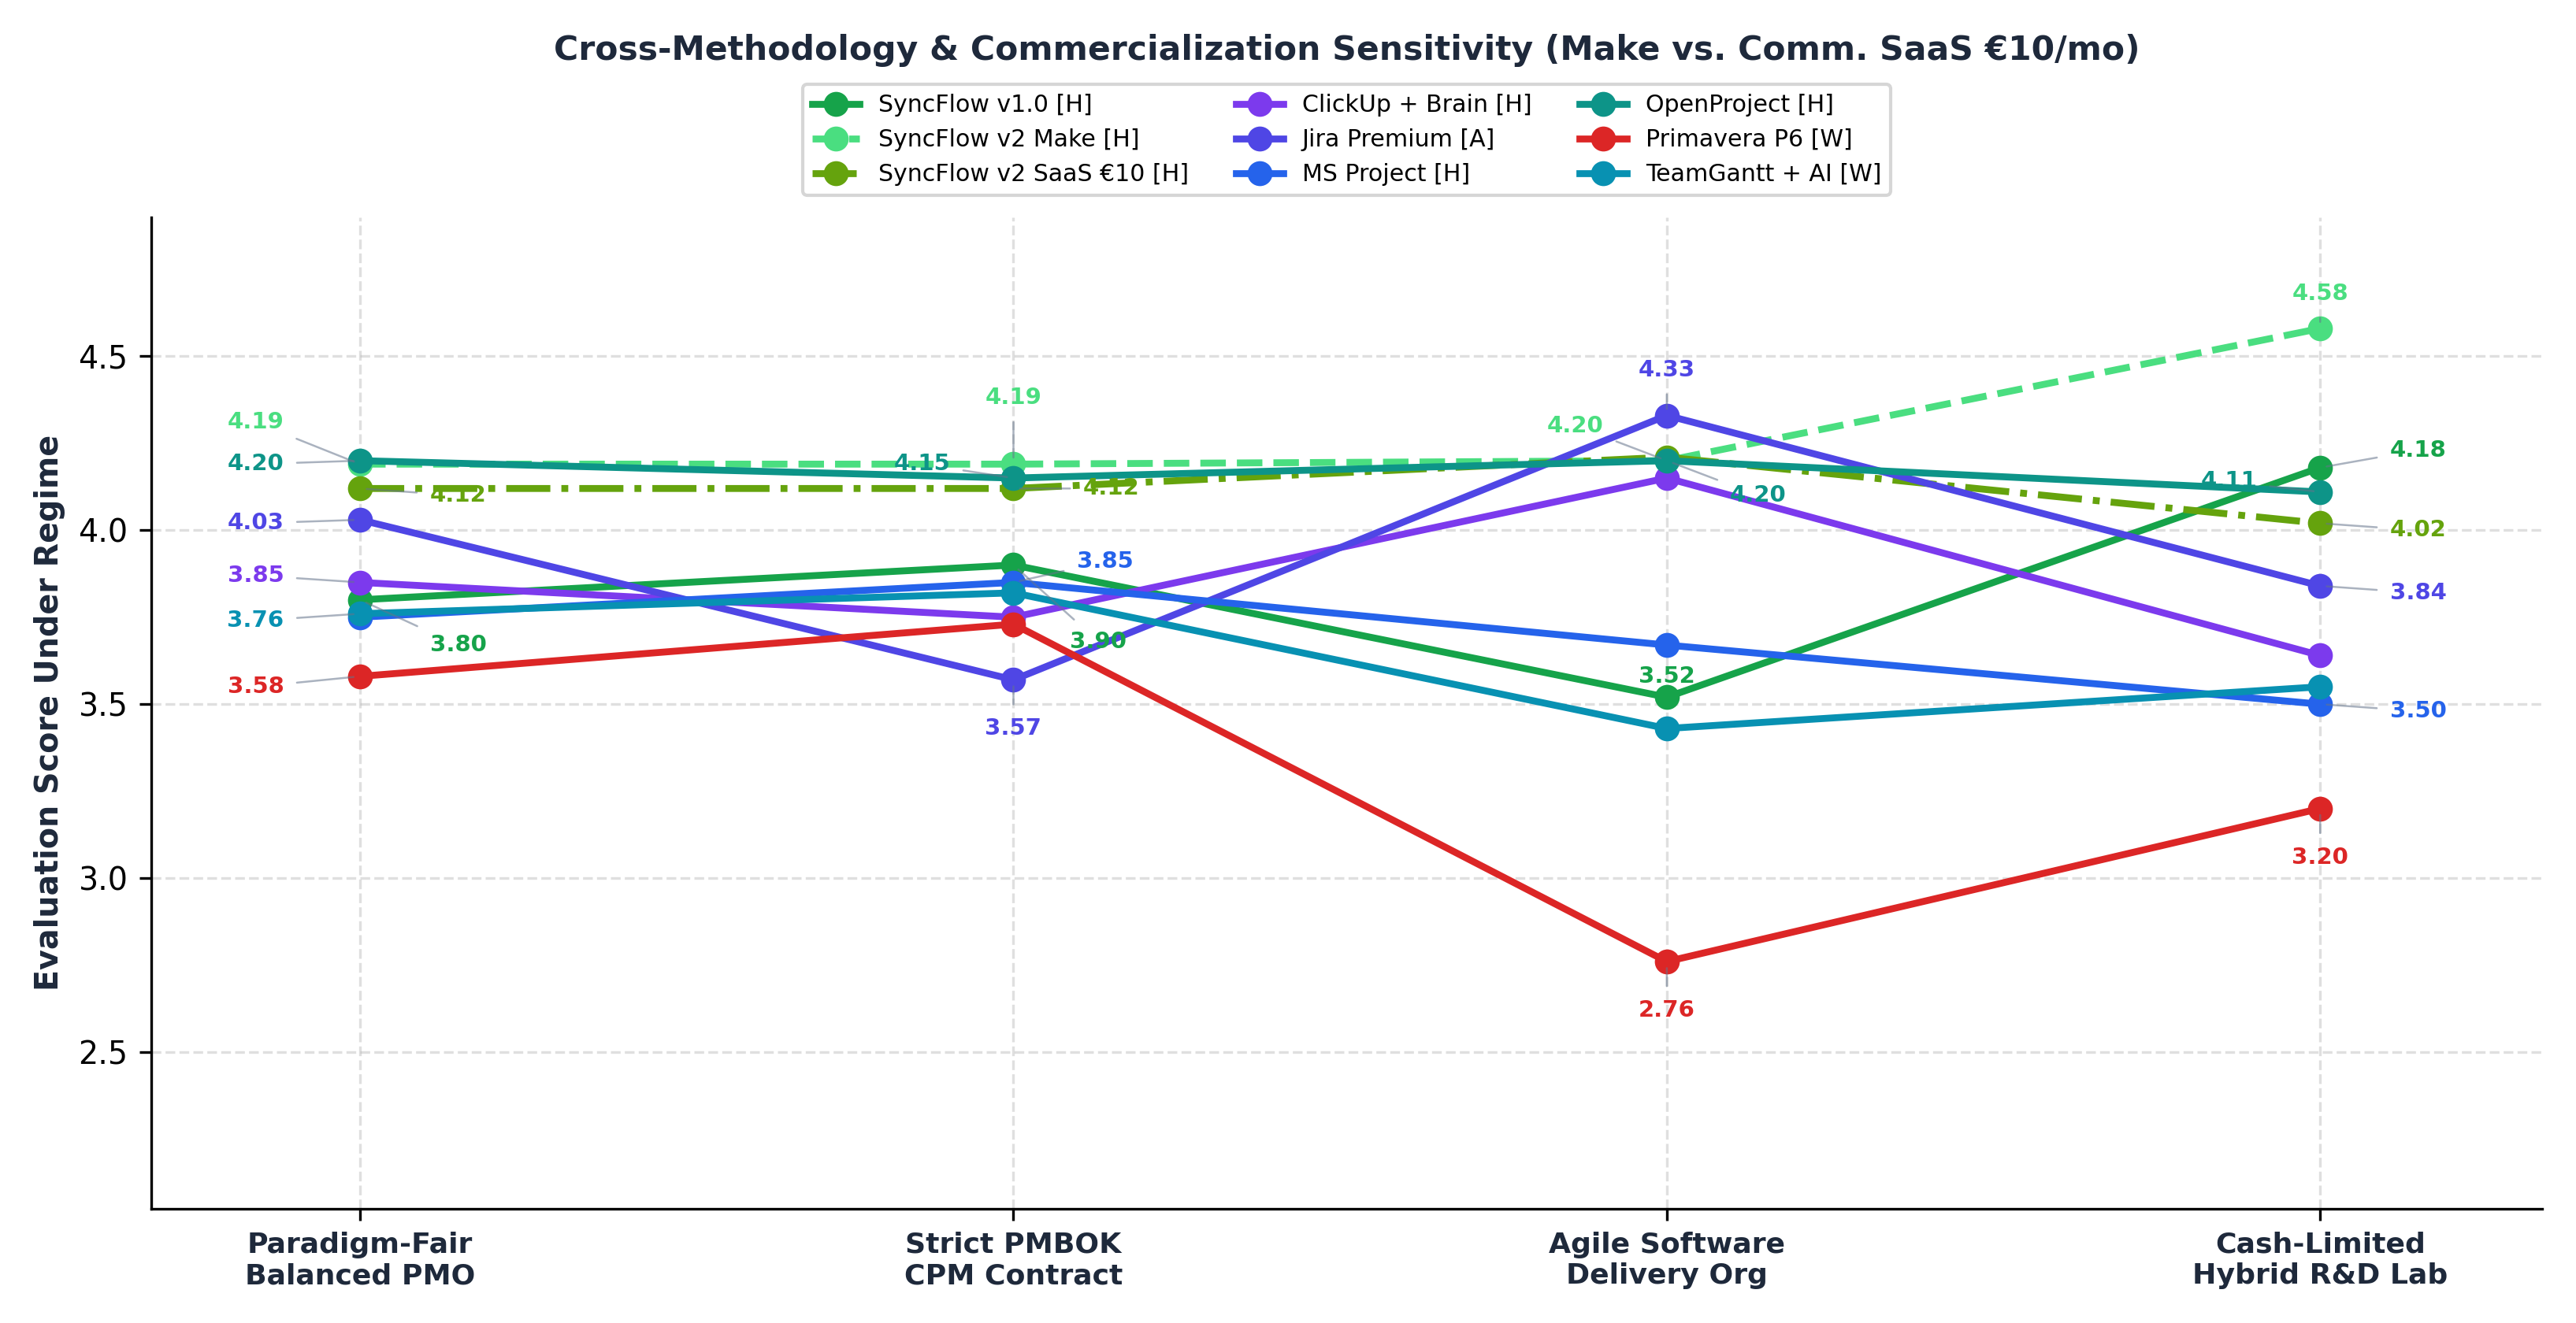
\includegraphics[width=1.0\textwidth]{images/va_sensitivity_scenarios.png}
    \caption*{Cross-methodology and commercialization sensitivity across Internal Make, Commercial SaaS (€10/mo), and commercial rivals.}
\end{figure}

Three clear behavioral patterns emerge from the sensitivity curves:
\begin{itemize}[itemsep=1pt,topsep=1pt]
    \item \textbf{Balanced Dominance vs. Strict CPM Shifts}: \textit{OpenProject Cloud} narrowly edges \textit{SyncFlow v2.0 (Make)} under Balanced PMO (4.20 vs. 4.19), but \textit{SyncFlow v2.0 (Make)} takes \#1 under Strict CPM (4.19 vs. 4.15). Baseline \textit{SyncFlow v1.0} advances significantly under Strict CPM (3.80 $\to$ 3.90, securing Rank \#2 ahead of \textit{Microsoft Project} at 3.85 and \textit{ClickUp} at 3.75). By contrast, \textit{Jira Premium} loses its Agile sprint advantage and drops from \#2 in Fair (4.03) to \#8 under Strict CPM (3.57);
    \item \textbf{Pure Agile Specialization}: When sprint delivery drives procurement, \textit{Jira Premium} climbs to \#1 (4.33), ahead of \textit{SyncFlow v2.0 SaaS} (4.21), \textit{SyncFlow v2.0 Make} (4.20), and \textit{OpenProject} (4.20), while strictly Waterfall \textit{Oracle Primavera P6} falls to 2.76;
    \item \textbf{Internal Custody Advantage in Self-Funded Labs}: Removing commercial subscription overhead boosts \textit{SyncFlow v2.0 (Make)} to 4.58 (\#1) and lifts baseline \textit{SyncFlow v1.0} (4.18) into \#2 above \textit{OpenProject} (4.11). Meanwhile, \textit{SyncFlow v2.0 (Comm. SaaS)} settles at \#4 (4.02) because recurring €10/seat fees remain mandatory even for technical teams.
\end{itemize}

\newpage

\section{Feasibility of Private Language Model Infrastructure}
\subsection{Architectural Paradigms for Personal Language Models}
To mitigate public cloud API quota throttling ($R_2$) and eliminate third-party data transmission risks ($R_3$), organizations may evaluate deploying a dedicated in-house language model system for \textit{SyncFlow}'s NLP operations (Text-to-WBS, PERT estimation, and dependency extraction). 

Building an in-house language model infrastructure involves three distinct technical approaches:
\begin{itemize}[itemsep=1.5pt,topsep=1.5pt]
    \item \textbf{Pre-Training from Scratch}: Foundational base pre-training requires $>10^{23}$ FLOPs, petabyte-scale web corpora, and millions of euros in compute, making it technically irrational for a 25-user suite;
    
    \vspace{1mm}
    
    \item \textbf{Domain Fine-Tuning (QLoRA)}: Adapting open weights via Low-Rank Adaptation (LoRA, rank $r=16$) on synthetic WBS trees costs under €20 in compute ($\approx 8$ GPU-hours on RTX 4090), conditioning the model on strict Pydantic schemas;
    
    \vspace{1mm}
    
    \item \textbf{Open-Weights Serving with Guided Decoding}: Serving an open-weights checkpoint via \texttt{vLLM} or \texttt{Ollama} with grammar-guided decoding (e.g., Outlines or XGrammar) forces the model to strictly adhere to \textit{SyncFlow}'s schema.
\end{itemize}

\vspace{4mm}

\subsection{Parameter Thresholds for Operational Effectiveness}
Scheduling calculations require exact JSON syntax, acyclic graph topology, and realistic PERT variance. Evaluating model performance across parameter classes reveals a clear operational threshold:
\begin{itemize}[itemsep=1.5pt,topsep=1.5pt]
    \item \textbf{Sub-7B Architectures (e.g., Qwen-2.5 7B)}: Executable on consumer hardware ($<12\text{ GB}$ VRAM), but empirical benchmarks reveal unacceptable schema dropouts ($\approx 28\%$ JSON syntax failures), cyclic dependency errors, and uncalibrated PERT variance;
    
    \vspace{1mm}
    
    \item \textbf{14B Architectures (e.g., Qwen-2.5 14B)}: \textbf{The optimal operational threshold}. Dense 14B models exhibit emergent reasoning for hierarchical deliverable breakdowns and acyclic graph construction ($>96\%$ schema adherence). Crucially, unquantized \textbf{FP16 is technically infeasible} on a single 24\,GB GPU: storing 14 billion parameters at 2 bytes per weight requires $14 \times 10^9 \times 2\text{ bytes} = \mathbf{28\text{ GB}}$ for model weights alone, exceeding physical VRAM before runtime buffers or Key-Value (KV) cache are allocated.
    
    However, \textbf{INT8 quantization} represents a highly viable configuration on a 24\,GB GPU (such as an NVIDIA RTX 4090 or A10G):
    \begin{itemize}[itemsep=1pt,topsep=1pt]
        \item \textit{Quantization Method}: 8-bit weight-only quantization via \textbf{AWQ (W8A16)} or \textbf{GPTQ INT8}, served via \texttt{vLLM} with PagedAttention;
        \item \textit{Memory Allocation}: The INT8 weights occupy $\approx 14.7\text{ GB}$. Allocating $\approx 1.8\text{ GB}$ for PyTorch/CUDA runtime overhead and activations leaves $\mathbf{\approx 7.5\text{ GB}}$ of dedicated VRAM exclusively for dynamic KV cache;
        \item \textit{Context Window and Batch Size}: Under Grouped-Query Attention (GQA) with an FP16 KV cache ($\approx 0.20\text{ MB/token}$), a standard 4,096-token WBS scheduling prompt consumes $\approx 0.80\text{ GB}$ per stream. The 7.5\,GB KV buffer reliably supports concurrent batch sizes of $\mathbf{B = 1\text{ to }4}$ without out-of-memory risk. For an internal 25-user PMO where requests arrive intermittently, batch size $B=1\text{--}2$ delivers immediate response at zero token cost.
    \end{itemize}
    
    \vspace{1mm}
    
    \item \textbf{32B--70B Architectures (e.g., Qwen-2.5 32B)}: Reaches near-perfect schema compliance ($>99\%$), but requires multi-GPU hardware (dual RTX 4090 or datacenter A100/H100), doubling CapEx and thermal load without yielding proportional utility for CPM math.
\end{itemize}

\subsection{Rigorous Cost Analysis for Private Inference}
Deploying a dedicated 14B parameter inference node requires accounting for upfront hardware acquisition (CapEx) and continuous electrical and maintenance overhead (OpEx) over a 36-month horizon, benchmarked against the public cloud API baseline:

\begin{table}[H]
\centering
\scriptsize
\setlength{\tabcolsep}{4pt}
\renewcommand{\arraystretch}{1.18}
\caption*{Three-Year Cost Comparison Across Cloud AI APIs versus Private On-Premise LLM Infrastructure.}
\begin{tabularx}{\textwidth}{>{\raggedright\arraybackslash}p{3.2cm} c c c >{\raggedright\arraybackslash}X}
\toprule
\textbf{Deployment Model} & \textbf{Hardware CapEx} & \textbf{3-Year OpEx} & \textbf{36-Mo TCO} & \textbf{Operational Trade-off} \\
\midrule
\textbf{Google Gemini 3.8 Flash} & \textbf{€0} & \textbf{€120} & \textbf{€120} & Lowest cost. Depends on external network connectivity and cloud terms. \\
\textbf{On-Premise 14B (Single GPU)} & €3,800 & €2,378 & €6,178 & Total air-gapped data sovereignty. Requires local server maintenance. \\
\textbf{Cloud Dedicated (AWS A10G)} & €0 & €5,940 & €5,940 & Zero CapEx, 40h/wk scheduled uptime. Incurs monthly cloud commitment. \\
\textbf{Cloud Dedicated (24/7 AWS)} & €0 & €24,840 & €24,840 & High availability cloud hosting. Exorbitant recurring OPEX commitment. \\
\textbf{On-Premise 70B (Dual GPU)} & €7,500 & €4,650 & €12,150 & Frontier reasoning quality. Excessive CapEx and power consumption. \\
\bottomrule
\end{tabularx}
\end{table}

\noindent \textbf{Financial Derivation}: The dedicated on-premise 14B system assumes a workstation server (€1,800) paired with an NVIDIA RTX 4090 24\,GB GPU (€2,000), yielding $\text{CapEx} = \text{€3,800}$. Continuous duty-cycle power consumption ($\approx 280\text{ W}$ average at €0.25/kWh) totals €613/year (€1,838 over 36 months), with €540 budgeted for system maintenance ($\text{OpEx} = \text{€2,378}$), producing $\text{TCO}_{\text{3yr}} = \mathbf{\text{€6,178}}$.

\noindent \textbf{Strategic Verdict}: At €120 over 36 months, \textbf{Google Gemini 3.8 Flash is $\approx 51\times$ less expensive} than a personal 14B LLM node. Constructing a personal LLM system is economically irrational for standard PMOs, but technically viable and justified strictly when sovereign compliance, defense air-gapping, or strict privacy regulations forbid cloud API utilization.

\vspace{4mm}

\section{Portability Exit Strategy}
Because all data schemas and scheduling logic remain self-contained, migrating off \textit{SyncFlow} carries minimal switching friction:
\begin{itemize}[itemsep=1.5pt,topsep=1.5pt]
    \item \textbf{Open JSON Data Export}: Project records export cleanly via \texttt{mongodump} or standard BSON/JSON tools for PostgreSQL or custom pipelines;
    \item \textbf{Isolated AI Adapter}: Generative AI calls sit inside one module, so swapping Gemini for OpenAI, Anthropic, or Ollama leaves CPM, PERT, and EVM logic untouched;
    \item \textbf{Offline Core \& Local Assets}: Deterministic scheduling works without internet APIs, and vendoring both JS chart libraries enables full air-gapped Docker deployment.
\end{itemize}

